\newpage
\section{Risultati Sperimentali}
\subsection{Sintesi}
Una volta eseguita la sintesi con successo sono stati analizzati 2 principali report:
\begin{itemize}
    \item \textbf{report\_timing} - risultati discussi nella Sezione \ref{Conclusione}
    \item \textbf{report\_utilization} - discusso di seguito
\end{itemize}

La rete ottenuta ha le seguenti caratteristiche: 
\begin{itemize}
    \item 138 Flip Flop - utilizzati per registri ad 8 e 16 bit e per memorizzare i 26 stati della macchina a stati con una codifica One-Hot
    \item  188 LUT
    \item  0 Latch - per evitare l'inferenza di Latch sono sempre stati inizializzati i segnali con un valore di default
\end{itemize}

Di seguito é riportato lo schema della rete realizzato da vivado:
%immagini
\begin{figure}[h!]
    \centering
    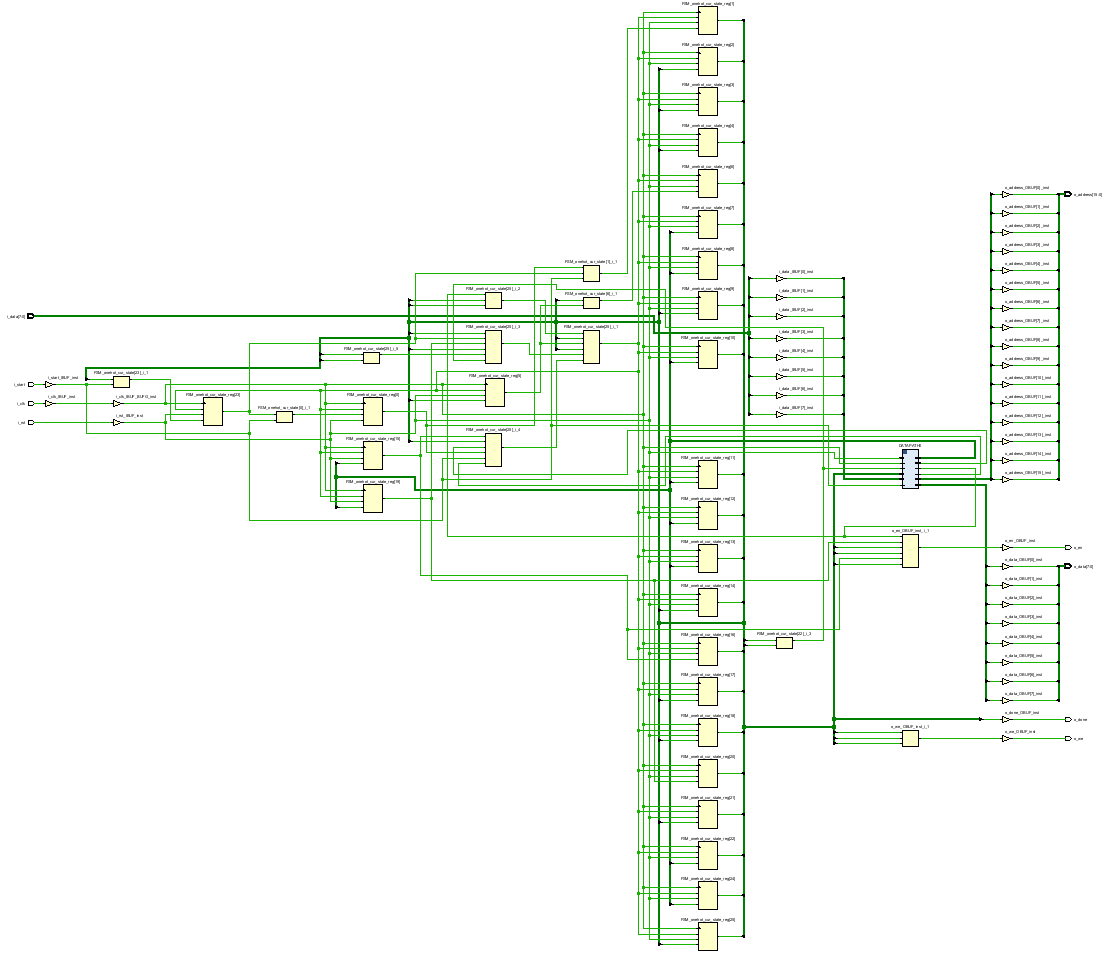
\includegraphics[scale = 0.54]{Figure/Sintesi}
    \caption{Schema del circuito sintetizzato}
    \label{Sintesi}
\end{figure}

\clearpage

\subsection{Simulazione}
Per verificare il corretto funzionamento del componente realizzato sono stati utilizzati diversi \textit{test bench} al fine di testare il comportamento, in Pre e Post sintesi, nella normale esecuzione e nei possibili casi limite.

Dopo aver appurato che il componente riuscisse a gestire semplici \textit{test bench} è stato sottoposto a 2 test per stressarne funzionalità e comportamento: 
\begin{itemize}
    \item il primo composto da una sequenza di 10 000 immagini di dimensione massima prefissata di 16 pixel per stressare il componente sotto il punto di vista dei reset;
    \item il secondo composto da una sequenza di 2000 immagini di dimensione massima prefissata di 128 pixel per stressare lettura e scrittura di grandi quantitá di dati in memoria e la gestione degli indirizzi in uscita.
\end{itemize}

I casi di test appena descritti hanno anche consentito di testare i casi limite, sia all'inizio del programma che all'interno di una serie di numerose altre operazioni, per assicurarsi della loro stabilità.

%%qui mettere una parte in cui descriviamo e mettiamo immagini di test di casi limite, immagini da 0 1 2 pixels
Abbiamo inoltre realizzato dei TB appositi per testare in maniera più specifica i casi limite di:
\begin{itemize}
    \item immagini di dimensione 0;
    \item immagini di dimensione 1;
    \item immagini di dimensione 2;
    \item immagini completamente bianche ;
    \item immagini completamente nere;
    \item immagini con pixel massimo '255' e pixel minimo '0' (con una conseguente non-necessità di equalizzare l'immagine);
\end{itemize}
che come spiegato in precedenza sono stati gestiti con un percorso di controllo alternativo della macchina a stati.

Di seguito riportiamo immagini e discussione di alcuni casi:
\subsubsection{Immagini di dimensione 0}

Nell'immagine (Figura \ref{0}) si può osservare che, come ci si aspetta, il segnale \texttt{finish} (che assume valore 0 solo nel momento in cui l'uscita di \texttt{registro\_TS} risulta essere != 0) rimane costante ad 1.
Questo consente di percorrere, partendo da S6, la sequenza di stati appositamente pensata per questo caso specifico.

\begin{figure}[h!]
    \centering
    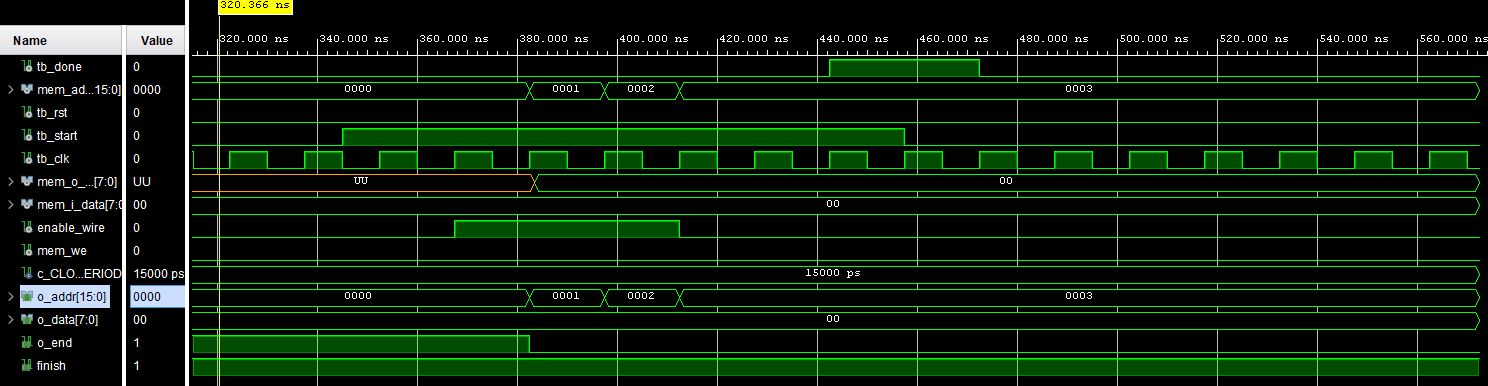
\includegraphics[scale = 0.3919]{Figure/TB_0x0.PNG}
    \caption{Screenshot caso particolare 1}
    \label{0}
\end{figure}

\clearpage

\subsubsection{Immagini di dimensione 1}
Nell'immagine (Figura \ref{1}) si può osservare che, appena dopo aver letto i primi 2 indirizzi di memoria e calcolato il numero di pixel, il segnale \texttt{o\_end} rimane alto (per via del comparatore che controlla che l'uscita di \texttt{regTS+1} sia uguale a 2) consentendo anche in questo caso di seguire il percorso di controllo dedicato. 


\begin{figure}[h!]
    \centering
    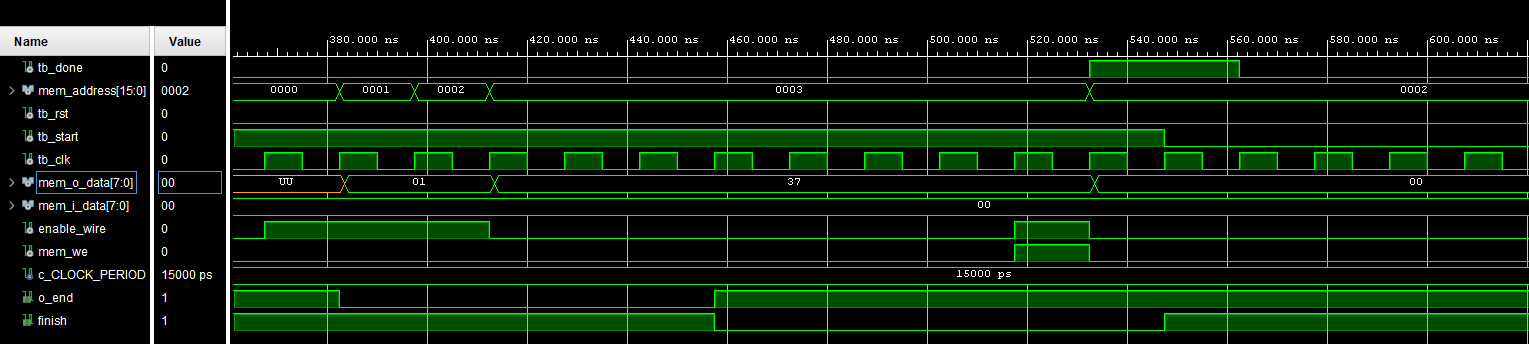
\includegraphics[scale = 0.3793]{Figure/TB_1x1.PNG}
    \caption{Screenshot caso particolare 2}
    \label{1}
\end{figure}

\subsubsection{Immagini di dimensione 2} %TODO

In questo ultimo caso (Figura \ref{2}) é possibile notare che il segnale \texttt{o\_end} viene portato alto prima rispetto al caso standard\footnote{\texttt{o\_end} viene posto a 1 almeno un ciclo di CK dopo la lettura del secondo pixel} in modo tale da evitare la lettura delle celle di memoria immediatamente successive (che sono le prime a non contenere l'immagine) per poi riabbassarlo e collegarsi al flow di controllo standard.
\begin{figure}[h!]
    \centering
    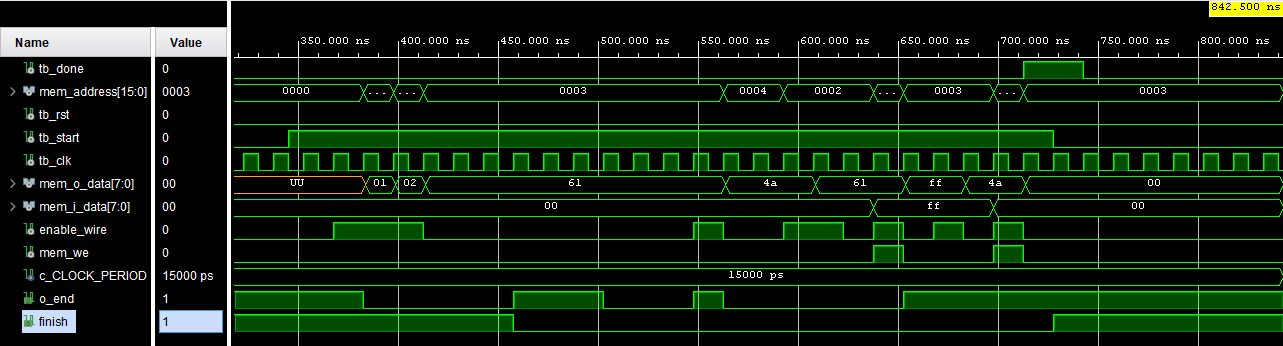
\includegraphics[scale = 0.45]{Figure/TB_2x1.PNG}
    \caption{Screenshot caso particolare 3}
    \label{2}
\end{figure}

\clearpage
